\documentclass{article}

%package setup
\usepackage{graphicx}
\graphicspath{ {./images/} }
\usepackage{amsmath}
\usepackage{fancyhdr}
\usepackage[margin=1in]{geometry}
\usepackage{subcaption}
\usepackage{comment}
\usepackage[hidelinks]{hyperref}
\usepackage{enumitem}
\usepackage{float}
\usepackage{textcomp, gensymb}
\usepackage{caption}
\setlength\parindent{0pt}


% \pagestyle{fancy}
% \fancyhf{} % Clear header/footer settings
% \rhead{\thepage} % Page number on the right in the header
% \lhead{ASE 375 Final Project Proposal} % Your lab report title on the left

% \title{Propeller Twist Efficiency}
% \author{Group 6: Andrew Doty, Andres Suniaga, Dennis Hom}

\begin{document}
\begin{flushleft}
    \small{ASE 375 Group 6 (14115): Andrew Doty, Andres Suniaga, Dennis Hom}\\[2mm]    
    \Large{\textbf{Project Proposal: Propeller Twist Efficiency}}\\[2mm]
\end{flushleft}
% \maketitle
% \begin{titlepage}
  % \centering
  % 
\includegraphics[height=2.5cm]{ase-logo-formal.png}  % Adjust the height as needed
  % \vspace{1cm}  % Add some vertical space
 
%   \Large \textbf{ASE 375 Electromechanical Systems}\\
%   \large \textbf{Section 14115}\\
%   \vspace{0.5cm}
%   \textbf{Monday: 3:00 - 6:00 pm}\\
 
%   \vspace{1cm}
 
%   \hrule
%   \vspace{0.5cm}
 
%   \Huge \textbf{Final Project Proposal: \\
%                 Propeller Twist Efficiency}
%  \Huge \textbf{}\\
 
%   \vspace{0.5cm}
%   \hrule
 
%   \vspace{1cm}
 
%   \normalsize \textbf{Group 6: Andrew Doty, Andres Suniaga, Dennis Hom}\\
%   \normalsize \textbf{Due Date: 04/01/2024}
 
% \end{titlepage}

\section{Question}
\textbf{How does propeller twist affect efficiency?} Twist defines the angle of incidence of the propeller. This varies from the hub to the tip of the prop due to the different speeds along the blade as the propeller spins.
\section{Experiment}
How will we determine the propeller's efficiency? Using a thrust stand designed to mount a Brushless DC Motor and Speed Controller, we will measure the thrust force and the power used. The speed of the motor will be controlled via PWM signal generator communicating through the speed controller. For consistency, the same PWM signal will be supplied for all tests. Using a load cell placed at the root of our stand (beam as shown in \ref{fig:finalsetup}) we will measure the propeller's thrust. For accurate data collection we will calibrate this load cell to measure this thrust applied at the tip of the stand. With the DAQ, we can gather this load cell data.  With a power supply, we can ensure that the same input voltage is supplied and from a watt-meter we can gather the electrical power consumption.
\begin{figure}[H]
    \centering
    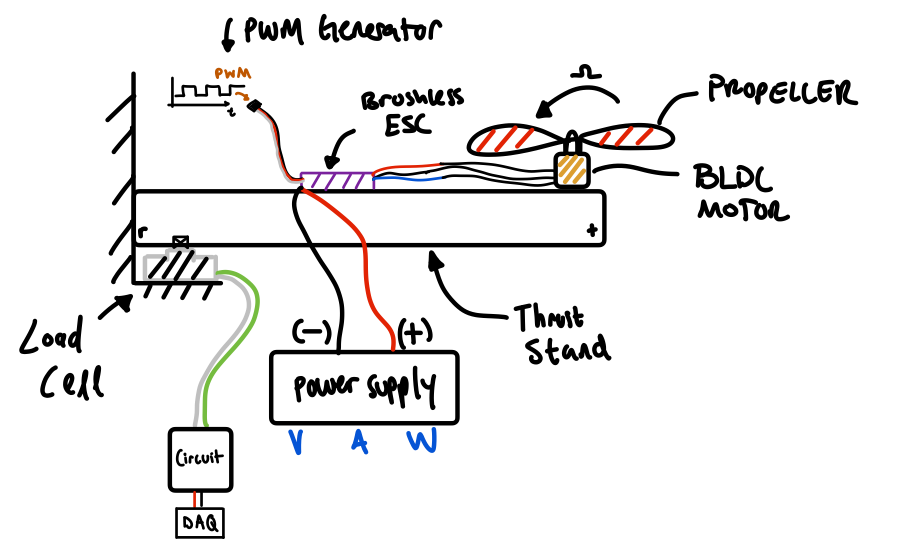
\includegraphics[width = 0.5\textwidth]{finalproject/EMech_FinalExperiment_IdeaSetup_Updated.png}
    \caption{Hypothetical Experiment Setup}
    \label{fig:finalsetup}
\end{figure}
We will experiment with a number of propellers of different twist but same diameter. With a ratio of the propeller thrust and electrical power consumption we can determine the efficiency of the propeller and how it is affected by twist.
\section{List of Equipment}
\begin{enumerate}
    \item Tension Link Load Cell, along with required connections and components for DAQ 
    \item BLDC Motor with the proper rated Brushless Electronic Speed Controller 
    \begin{itemize}
        \item Stator diameter and height and $\text{K}_{\text{v}}\; [\frac{
        \text{RPM}}{\text{V}}]$ to be determined.
    \end{itemize}
    \item Power Supply or 3-6S Lithium-Ion/Polymer battery, with Voltmeter, Ammeter, and Watt-meter
    \item PWM Wave Generator or PWM/Servo Tester
    \item 3-5 Two-Blade Propellers of same diameter (dependent on the motor specifications) and different twist
    \item Thrust Stand with mounting for BLDC Motor and Placement of Load Cell
\end{enumerate}
\end{document}
